\documentclass[11pt]{article}

\pdfminorversion=4

% use packages
\usepackage[utf8]{inputenc}
\usepackage{amsmath}
\usepackage{amsthm}
\usepackage{amsfonts}
\usepackage{amscd}
\usepackage{amssymb}
\usepackage{natbib}
\usepackage{url}
\usepackage[table,xcdraw,usenames]{xcolor}
%\usepackage[usenames]{color}

\usepackage{graphicx}
\usepackage{subcaption}
\usepackage{mathtools}
\usepackage{enumitem}
\usepackage{authblk}
\usepackage{bm}
\usepackage{comment}
\usepackage{pdfpages}

\usepackage{hyperref}
\usepackage{caption}
\usepackage{float}
%\usepackage[caption = false]{subfig}
\usepackage{tikz}
\usepackage{multirow}
\usepackage[linesnumbered, ruled,vlined]{algorithm2e}
\usepackage{pdflscape}
\usepackage{etoolbox}

%\AtBeginEnvironment{align}{\setcounter{equation}{0}} % https://tex.stackexchange.com/questions/349247/how-do-i-reset-the-counter-in-align

% margin setup
\usepackage{geometry}
\geometry{margin=0.8in}

% function definition
\newcommand{\V}{\textbf{V}}
\newcommand{\weight}{\pi}
\newcommand{\ret}{\textbf{r}}
\newcommand{\y}{\textbf{y}}
\newcommand{\w}{\textbf{w}}
\newcommand{\x}{\textbf{x}}
\newcommand{\dbf}{\textbf{d}}
\newcommand{\X}{\textbf{X}}
\newcommand{\Y}{\textbf{Y}}
%\newcommand{\L}{\textbf{L}}
\newcommand{\Hist}{\mathcal{H}}
\newcommand{\Prob}{\mathbb{P}}
\def\mbf#1{\mathbf{#1}} % bold but not italic
\def\ind#1{\mathrm{1}(#1)} % indicator function
\newcommand{\simiid}{\stackrel{iid}{\sim}} %[] IID 
\def\where{\text{ where }} % where
\newcommand{\indep}{\perp \!\!\! \perp } % independent symbols
\def\cov#1#2{\mathrm{Cov}(#1, #2)} % covariance 
\def\mrm#1{\mathrm{#1}} % remove math
\newcommand{\reals}{\mathbb{R}} % Real number symbol
\def\t#1{\tilde{#1}} % tilde
\def\normal#1#2{\mathcal{N}(#1,#2)} % normal
\def\mbi#1{\boldsymbol{#1}} % Bold and italic (math bold italic)
\def\v#1{\mbi{#1}} % Vector notation
\def\mc#1{\mathcal{#1}} % mathical
\DeclareMathOperator*{\argmax}{arg\,max} % arg max
\DeclareMathOperator*{\argmin}{arg\,min} % arg min
\def\E{\mathbb{E}} % Expectation symbol
\def\mc#1{\mathcal{#1}}
\def\var#1{\mathrm{Var}(#1)} % Variance symbol
\def\checkmark{\tikz\fill[scale=0.4](0,.35) -- (.25,0) -- (1,.7) -- (.25,.15) -- cycle;} % checkmark
\newcommand\red[1]{{\color{red}#1}}
\def\bs#1{\boldsymbol{#1}}
\def\P{\mathbb{P}}
\def\var{\mathbf{Var}}
\def\naturals{\mathbb{N}}
\def\cp{\overset{p}{\to}}
\def\clt{\overset{\mathcal{L}^2}{\to}}

\setcounter{tocdepth}{4}
\setcounter{secnumdepth}{4}

\newtheorem{corollary}{Corollary}
\newcommand{\ceil}[1]{\lceil #1 \rceil}
\newcommand{\norm}[1]{\left\lVert#1\right\rVert} % A norm with 1 argument
\DeclareMathOperator{\Var}{Var} % Variance symbol

\newtheorem{cor}{Corollary}
\newtheorem{lem}{Lemma}
\newtheorem{thm}{Theorem}
\newtheorem{defn}{Definition}
\newtheorem{prop}{Proposition}
\theoremstyle{definition}
\newtheorem{remark}{Remark}
\hypersetup{
  linkcolor  = blue,
  citecolor  = blue,
  urlcolor   = blue,
  colorlinks = true,
} % color setup

% proof to proposition 
\newenvironment{proof-of-proposition}[1][{}]{\noindent{\bf
    Proof of Proposition {#1}}
  \hspace*{.5em}}{\qed\bigskip\\}
% general proof of corollary
  \newenvironment{proof-of-corollary}[1][{}]{\noindent{\bf
    Proof of Corollary {#1}}
  \hspace*{.5em}}{\qed\bigskip\\}
% general proof of lemma
  \newenvironment{proof-of-lemma}[1][{}]{\noindent{\bf
    Proof of Lemma {#1}}
  \hspace*{.5em}}{\qed\bigskip\\}

\allowdisplaybreaks

\title{Forecast Adjustment Under Shocks: A Unification}
\author{David Lundquist\thanks{davidl11@ilinois.edu}, Daniel Eck\thanks{dje13@illinois.edu} }
\affil{Department of Statistics, University of Illinois at Urbana-Champaign}
\date{\today}

\begin{document}

\maketitle

\begin{abstract} 
This work systematizes and unifies the rich landscape of model adjustment and model correction methods, with a special focus on forecast adjustment under the presence of shocks.


\end{abstract}

\section{Introduction}

For various modeling and prediction tasks in time series and panel data, the salient challenge is not predicting when an event will occur but what its direction, sign, magnitude, duration, correlation structure, or after-effects will be. This is not to say that predicting when a given event will occur is easy. In some cases, it may be difficult or impossible, and in those situations in particular, preparing for the shock is the best one can hope for.

This work focuses on model adjustment amid structual shocks that undermine the reliability of the  model at hand.  Forecasting under anticipated shocks raises unavoidable questions: should the forecast model be abandoned in favor of a discretionary or ad-hoc or one-off adjustment?  Does the does the discretion of a forecaster rule out a quantitative method for making the adjustment?  What is the ultimate purpose of the adjustment, and how it is to be used?  For how long is the adjustment necessary or reliable?

Herein we systematize and unify a range of conceptual approaches and tools that have developed across the broad ecosystem of the econometric and forecasting literatures.  Additionally, we delineate a specific type of forecasting problem called post-shock forecasting, which we broadly define as forecasting when the a shock intervenes.\\

difference between discretionary and automated \citep{hendry1994theory}\\

Setting the model back on track \citep{hendry1994theory}\\

what we are talking about here is not forecast combination, but there may be, nevertheless, a role for forecast combination: combining the forecasts generated by small differences in covariate and/or donor choice\\

The role and meaning of similarity\\

How important is a shared DGP?\\

Bias-variance tradeoff and MSE decomposition\\


Mismeasured data is discussed in \cite[p. 166]{hendry1994theory} as a motivator for intercept correction.  Could similarity-based correction help?\\

The forecast horizon --- does it matter?  If so, how so?  \cite{lin2021minimizing} has a one-period horizon.  \cite{clements1998forecasting}{p. 203} discuss how long to keep the forecast adjustment in place.  For a corrected ``slope parameter'', the effect of $h$ is not so clear.

\subsection{Literature Review}

Three Clements and Hendry books

\begin{itemize}
\item 1994
\item 1998
\item 1999
\end{itemize}

Quinton-Guerrera and Zhong

Evaluating a Model by Forecast Performance \cite{clements2005evaluating}
\begin{itemize}
  \item unconditional versus conditional
  \item internal versus external evaluation
  \item constancy versus adventitious
  \item skip
  \item 1step versus multi-horizon forecasts -- this is a relevant question to ask in the context of post-shocking forecasting: should we correct the earliest forecast and then allow the shock to propagate, or should we just correct each term in the horizon, h=1, 2,..., H?
\end{itemize}


\subsection{Model Adjustment Using Similarity-Based Parameter Correction: A Global Overview}

\begin{enumerate}
  \item a random object to forecast that depends on a linear specification
  \item a parametric model family shared by donors
  \item a correction term for the model family shared by donors
  \item a parametric specification for the correction term

  \item a reliable estimation procedure for the shared model
  \begin{enumerate}
  \item This should be straightforward
  \end{enumerate}
  \item a reliable estimation procedure for the correction term 
  \begin{enumerate}
    \item This might not be straightforward.  Some models like GARCH, for example, might deliver very noisy estimates for indicator variables that occur just once.
    \end{enumerate}
  \item a correction function that aggregates (i.e. maps) donor correction terms based on some notion of similarity
\end{enumerate}
Emphasize that there is a non-parametric version of the above: for example, one can use LSTM to predict each of the donor shocks, and then the residuals of those $n$ models can be weighted to arrive at a correction term.


\section{Setting}

\section{Model-Specific Considerations}

\subsection{ARIMA}
\subsection{GARCH}
\subsection{HAR}

\begin{figure}[h!]
  \begin{center}
    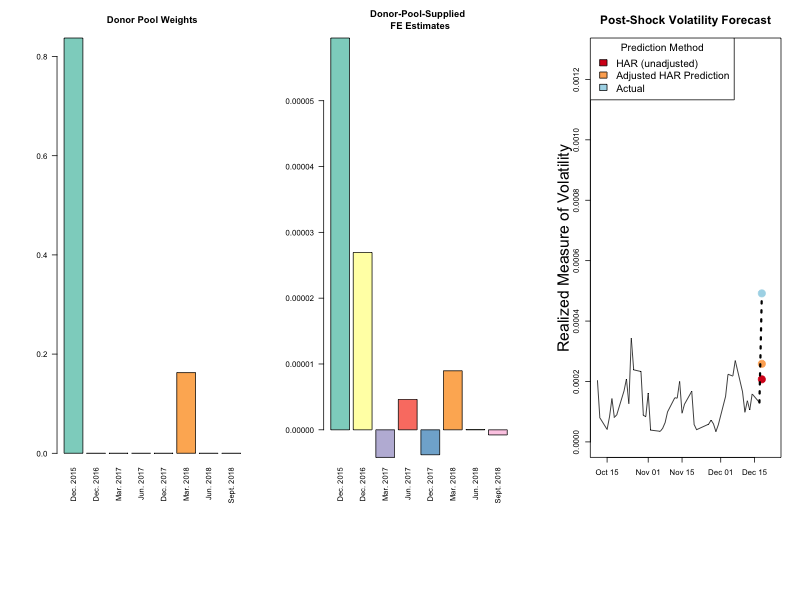
\includegraphics[scale=.4]{real_data_output_plots/savetime_SatJun151644072024__^VIX-^IRX-^XAU_^VIX_2018-12-18-2015-12-15-2016-12-13-2017-03-14-2017-06-13-2017-12-12-2018-03-20-2018-06-12-2018-09-25.png}
    \caption{Volatility series of six i.i.d. GARCH processes, each of which experiences a volatility shock, indicated with a red vertical line, at a uniformly distributed point in the set $\{756,...,2520\}$ of trading days, corresponding to between 3 and 10 years of daily trading data.}
    \label{fig:six_plots}
    \end{center}
  \end{figure}

\subsection{VAR}

\section{Real Data Examples}
\section{Discussion}

\begin{itemize}
  \item Binary Outcome Forecasts
  \item Density Forecasts
  \item Quantile Forecasts
\end{itemize}

\clearpage

\bibliographystyle{plainnat}
\bibliography{synthVolForecast}
 
\end{document}